\section{Transition systems for graph rewriting}

\subsection{Graph rewriting}

\begin{definition}[Category of simple graphs]
  We define the category of \emph{simple graphs} $\mathcal{G}$ where
  \begin{itemize}
  \item objects are graphs: $G = (V,E)$ with $V$ a set of nodes and $E$ a binary symmetric reflexive relation on nodes, representing the edges;
  \item morphisms $h:G_1\to G_2$ are functions on nodes $h_V:V_1\to V_2$ that preserve edges: $(s,t)\in E_1\implies (h_V(s),h_V(t))\in E_2$. We denote $h_E$ the function on edges: $h_E(s,t) = (h_V(s), h_V(t))$.
  \end{itemize}
  Denote $\varepsilon$ the empty graph.
\end{definition}

A mono is a morphism injective on nodes. A subgraph $S = (V_S,E_S)$ of $G$, is graph such that $V_S\subseteq V$ and $E_S\subseteq E$.

\begin{definition}[Pushout]
  The \emph{pushout} of the span $G_1\leftarrow O\rightarrow G_2$ is the cospan $G_1\rightarrow M\leftarrow G_2$ such that the following diagram commutes
  \[
  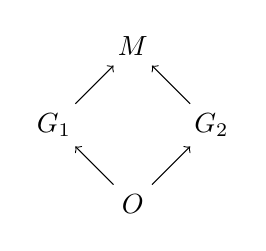
\begin{tikzpicture} %[scale=0.8]
    \node (o) at (0,-1) {\(O\)};
    \node (l1) at (-1,0) {\(G_1\)};
    \node (l2) at (1,0) {\(G_2\)};
    \node (m) at (0,1) {\(M\)};
    \draw [->] (o) --  (l1);
    \draw [->] (o) --  (l2);
    \draw [->] (l1) --  (m);
    \draw [->] (l2) --  (m);
  \end{tikzpicture}
  \]
  and such that for any other cospan $G_1\rightarrow M'\leftarrow G_2$ for which the diagram commutes, there is a unique morphism $M\to M'$:
  \[
  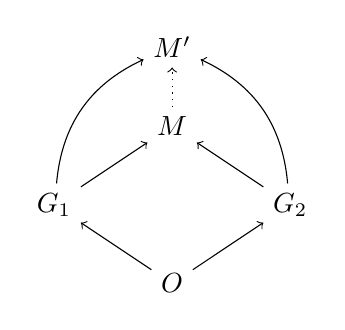
\begin{tikzpicture} %[scale=0.8]
    \node (mp) at (0,2) {\(M'\)};
    \node (o) at (0,-1) {\(O\)};
    \node (l1) at (-1.5,0) {\(G_1\)};
    \node (l2) at (1.5,0) {\(G_2\)};
    \node (m) at (0,1) {\(M\)};
    \draw [->] (o) --  (l1);
    \draw [->] (o) --  (l2);
    \draw [->] (l1) --  (m);
    \draw [->] (l2) --  (m);
    \draw [->] (l1) to [bend left] (mp);
    \draw [->] (l2) to [bend right] (mp);
    \draw [->, dotted] (m) -- (mp);
  \end{tikzpicture}
  \]
\end{definition}

\begin{property}
  \begin{itemize}
  \item The pushout is unique up to isomorphism.
  \item The pushout preserves monos: if $O\to G_i$ is a mono then $G_i\to M$ is also a mono.
  \end{itemize}
\end{property}

\begin{definition}[Double-pushout rewriting]
\label{def:dpo}
  Let $p = L\overset{l}{\leftarrow} K \overset{r}{\rightarrow} R$ be a span of injective morphisms, called a \emph{production} or a \emph{rule}. Let $M$ be a graph and $L\lemb M$ be an injective morphism in $M$, called \emph{a matching}.

  The \emph{double pushout transformation} consists in defining the graphs $D'$, called the \emph{context} graph, and the graph $N$ such that in the following diagram:
  \[
  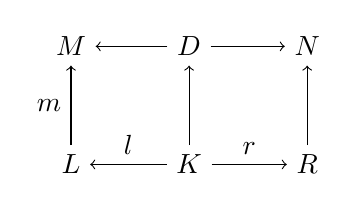
\begin{tikzpicture} %[scale=0.8]
    \node (l) at (-1.5,0) {\(L\)};
    \node (d) at (0,0) {\(K\)};
    \node (r) at (1.5,0) {\(R\)};
    \node (m) at (-1.5,1.5) {\(M\)};
    \node (d') at (0,1.5) {\(D\)};
    \node (n) at (1.5,1.5) {\(N\)};
    \draw [->] (d) -- node [above,midway] {\(l\)} (l);
    \draw [->] (d) -- node [above,midway] {\(r\)} (r);
    \draw [->] (d') -- (m);
    \draw [->] (d') -- (n);
    \draw [->] (l) -- node [left,midway] {\(m\)}  (m);
    \draw [->] (d) -- (d');
    \draw [->] (r) -- (n);
  \end{tikzpicture}
  \]
  the two squares are pushouts.
\end{definition}

  %We denote $L\action R$ the span $p:L\overset{l}{\leftarrow} K \overset{r}{\rightarrow} R$.
  The inverse rule is defined as $p^{-1} = R\overset{r}{\leftarrow} K \overset{l}{\rightarrow} L$.
  We write $M\overset{m,p}{\Rightarrow}N$ to denote the dpo rewrite of $M$ to $N$ of~\autoref{def:dpo}.
  We sometimes also write $L\overset{\mathit{id}_L,p}{\Rightarrow}R$ (or $L{\Rightarrow}R$) for
  %the production $p:L\action R$ and
  $\mathit{id}_L$ the identity morphism on $L$.

  %For any graph $G$ let us denote $V_G$ and $E_G$ the corresponding set of nodes and edges, respectively.

\begin{property}[Gluing conditions]
  Let $p = L\overset{l}{\leftarrow} K \overset{r}{\rightarrow} R$ be a production and let $L\overset{m}\lemb M$ be a matching in a graph $M$.
  Define the \emph{gluing points} and \emph{dangling points} as the two following sets:
  \begin{align*}
  \text{GP} &= l_V(V_K)\cup l_E(V_K)\\
  \text{DP} &= \{ v\in V_L \big| \exists e\in E_G\setminus m_E(E_L)\text{ s.t. }e=(v,\_)\text{ or }e=(\_, v)\}.
  \end{align*}
  Then DP $\subseteq$ GP iff there exists a unique $D$ such that $L\overset{m}{\rightarrow} M{\leftarrow} D$ is the pushout of the span $ L\overset{l}{\leftarrow} K {\rightarrow} D$.
\end{property}

Henceforth we only consider productions that satisfy the gluing condition.

\begin{remark}
Other graph rewriting techniques exists that allows production with dangling points. However, we are interested in reversible rules, and the DPO approach gives us the inverse of a rule in a straightforward way. We plan to extend the current work to rules with side effect in the future.
\end{remark}

\begin{definition}[Partial graph morphism]
  A partial morphism $g:L \pmorph R$ is a total morphism from the subgraph $\text{dom}(g)$ of $L$ to $R$, that is $g:L \supseteq \text{dom}(g) \to R$.
\end{definition}

\begin{definition}[Partial morphisms of productions~\cite{Ehrig:SPO}]
  Given a production $p:L\overset{l}{\leftarrow} K \overset{r}{\rightarrow} R$, its corresponding partial morphism, denoted $\spo(p):L\pmorph R$, is defined on $l(K)$ as $r\circ l^{-1}$ and undefined otherwise.
%  Similarly, for a partial morphism $p:L\leftarrow R$, a span $\dom(p):L\overset{l}{\leftarrow} \text{dom}(p) \overset{r}{\rightarrow} R$ where $l$ is the inclusion of $\text{dom}(p)$ in $L$ and $r$ is the restriction of $p$ to $\text{dom}(p)$.
\end{definition}
